%----------existing systems---------------------
\section{Existing Systems}
% ============================================================

In order to better understand existing digital solutions in agricultural trade, three representative digital platforms were analyzed.
The analyzed digital platforms take into account different approaches to digitalization in the agricultural trade market.

The purpose of this analysis is to identify its strengths and weaknesses in
order to properly position the proposed AgriGov Market platform:

% ============================================================
\subsection{Farmers Business Network (FBN) -- United States}

Farmers Business Network (FBN), which began operations in 2014 in the United States, is a private digital agricultural network that aims to improve price transparency and data sharing among farmers. The network, which has thousands of farmers across North America, offers price comparison services for farmers, direct selling options, agronomic information based on collective data, as well as financial services \cite{wolfert2017}.

\begin{figure}[H]
	\centering
	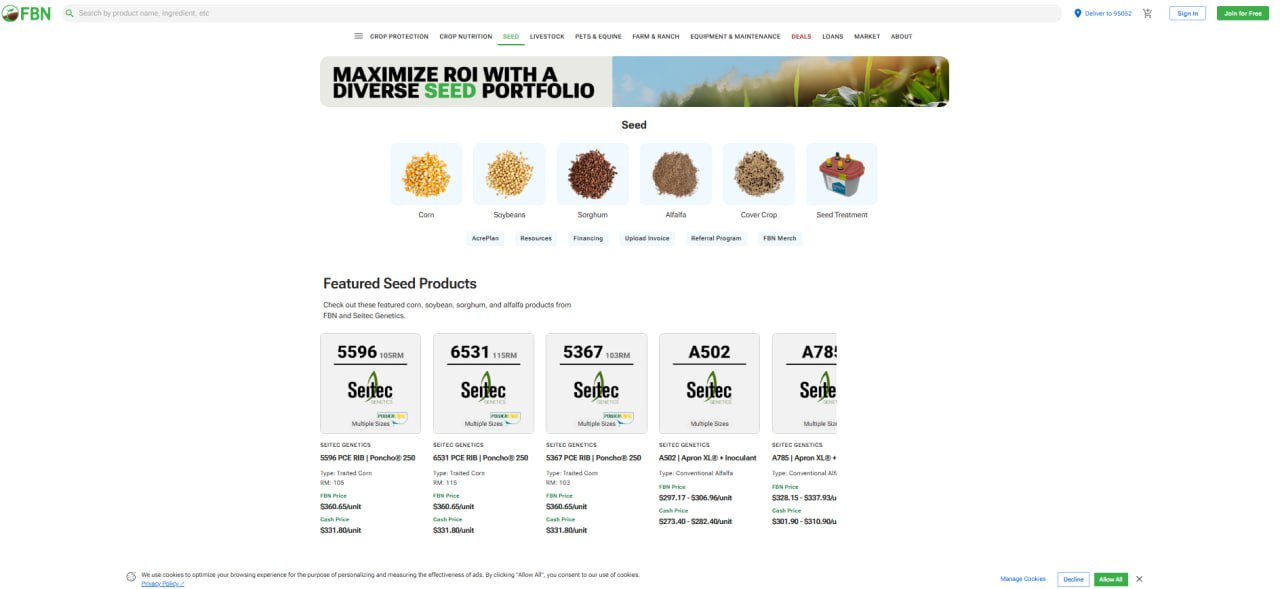
\includegraphics[width=0.8\textwidth]{images/existingHome/fbn_interface.png}
	\caption{FBN-Interface :https://www.fbn.com/}
	\label{fig:fbn}
\end{figure}

% ============================================================
\subsection{eNAM (Electronic National Agriculture Market) -- India}

Electronic National Agriculture Market (eNAM) is a government-driven project launched in 2016 to integrate Indian agricultural markets at a national level.
eNAM provides a link between Agricultural Produce Market Committees (APMCs) via an online trading system that allows nationwide bidding, quality assessment, and direct bank transfers for farmers.

As a government-driven project, eNAM is a remarkable institutional effort to promote and regulate agricultural trade.

\begin{figure}[H]
	\centering
	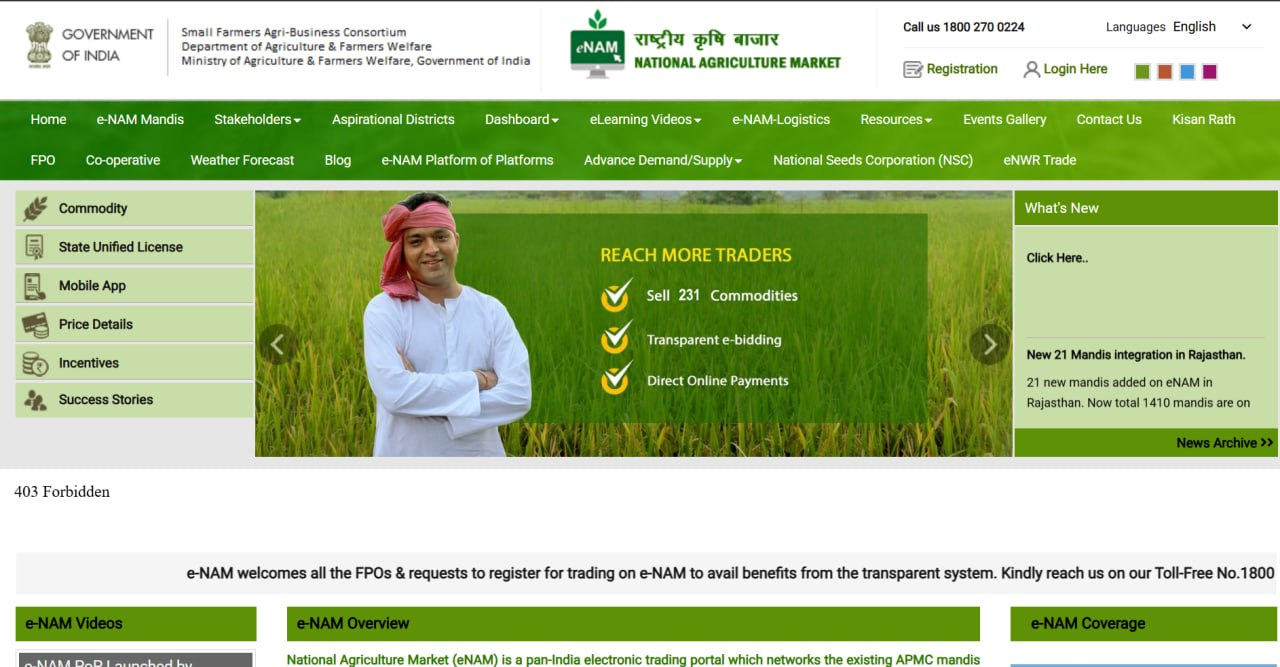
\includegraphics[width=0.8\textwidth]{images/existingHome/enam_interface.png}
	\caption{eNAM :www.enam.gov.in}
	\label{fig:enam}
\end{figure}

% ============================================================
% ============================================================
\subsection{Ghana Agriculture and Agribusiness Platform (GhAAP) -- Ghana}

The Ghana Agriculture and Agribusiness Platform (GhAAP) is a web-based platform developed in Ghana to support farmers and agribusiness actors through multiple digital services. The platform allows users to request farm services such as mechanization, spraying, and harvesting operations. 

It also connects farmers with agricultural extension agents who provide professional advice and technical support. In addition, the platform enables farmers to list and sell their agricultural products directly, while linking users to other commodity trading platforms to expand market access.

Through real-time information sharing, GhAAP improves coordination, transparency, and monitoring across the agricultural value chain.

\begin{figure}[H]
	\centering
	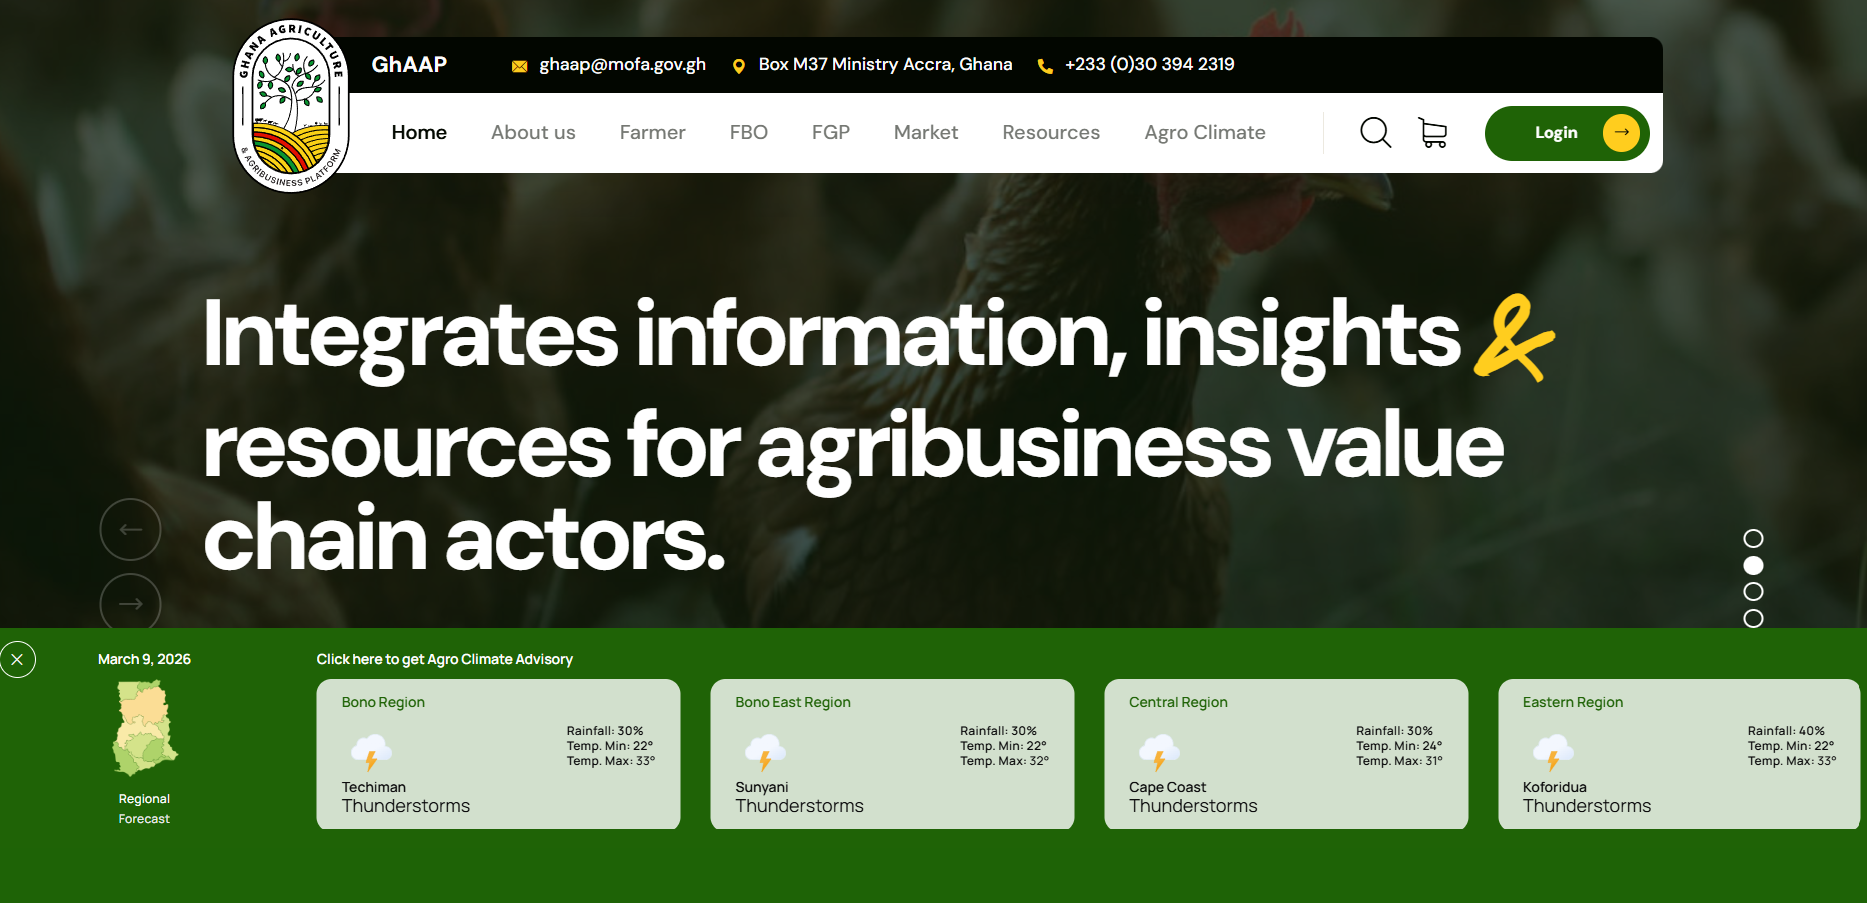
\includegraphics[width=0.8\textwidth]{images/existingHome/ghaap_interface.png}
	\caption{GhAAP: https://ghaap.com/}
	\label{fig:ghaap}
\end{figure}

% ============================================================

\subsection{Limitations and our solutions}
\begin{table}[H]
	\centering
	\begin{tabular}{|p{2.5cm}|p{2cm}|p{4.5cm}|p{4cm}|}
		\hline
		\textbf{System} & \textbf{Country} & \textbf{Strengths} & \textbf{Limitations} \\
		\hline
		FBN & USA & Price transparency, collaborative network, agronomic analytics & Paid model, no logistics integration, no government supervision \\
		\hline
		eNAM & India & Government-backed, national integration, quality testing, logistics module & Infrastructure gaps, digital divide, regulatory complexity \\
		\hline
		Ghana Agriculture and Agribusiness Platform (GhAAP) & Ghana & Farm services, extension advice, direct selling, links to other markets & National platform only, limited information on pricing mechanisms \\
		\hline
	\end{tabular}
	\caption{Comparative Analysis of Existing Systems}
	\label{tab:existing-systems}
\end{table}

Although Table \ref{tab:existing-systems} highlights the main characteristics of each platform, a deeper comparative analysis reveals important insights.

First, the studied systems adopt different operational models. FBN represents a \textbf{private and data-driven approach}, focusing on price transparency and analytics, but lacking institutional regulation. In contrast, eNAM follows a \textbf{government-driven model}, ensuring market integration and regulatory oversight, although it faces challenges related to infrastructure and system complexity. GhAAP, on the other hand, adopts a \textbf{service-oriented approach}, combining advisory services and market access, but remains limited in terms of scalability and pricing transparency.

Second, none of these platforms provides a \textbf{fully integrated solution}. While FBN lacks logistics and governance, eNAM struggles with accessibility and implementation constraints, and GhAAP does not offer advanced pricing mechanisms or national-level coordination.

These observations highlight a critical gap: the absence of a unified platform that combines \textbf{market transparency, logistics management, and governmental supervision} within a single system.

Therefore, AgriGov Market aims to address these limitations by proposing an integrated and institutional solution adapted to the Algerian context, ensuring better coordination between actors, improved price regulation, and enhanced transparency across the agricultural value chain.

% ============================================================
\subsubsection{Discussion}

In this context, AgriGov Market is positioned as an institutional and integrated digital platform tailored to Algeria. It combines product commercialization, logistics coordination, and regulatory supervision under the authority of the Ministry of Agriculture, aiming to ensure transparency, market stability, and modernization of the national agricultural value chain.




